% +------------------------------------------------------------------------+
% | CGAL User Manual: 
% +------------------------------------------------------------------------+
% |
% | 28.05.2008   Peter Hachenberger
% | 
\RCSdef{\ConvexDecomposition3Rev}{$Id$}
\RCSdefDate{\ConvexDecomposition3Date}{$Date$}
% +------------------------------------------------------------------------+

\ccParDims

\ccUserChapter{Convex Decomposition of Polyhedra \label{chapterConvexDecomposition3}}
\ccChapterRelease{\ConvexDecomposition3Rev. \ \ConvexDecomposition3Date}
\ccChapterAuthor{Peter Hachenberger}


\begin{ccPkgDescription}{3D Convex Hulls\label{Pkg:ConvexHull3}}
\ccPkgHowToCiteCgal{cgal:hs-ch3-07}
\ccPkgSummary{This package provides functions 
for computing convex hulls in three dimensions as well as functions
for checking if sets of points are strongly convex are not. One can
compute the convex hull of a set of points in three dimensions in one
of three ways: using a static algorithm, using an incremental
construction algorithm, or using a triangulation to get a fully
dynamic computation.}

\ccPkgDependsOn{All algorithms produce as output a \ccRef[3D Polyhedron]{Pkg:Polyhedron}. 
                The dynamic algorithms depend on \ccRef[3D Triangulations]{Pkg:Triangulation3}}
\ccPkgIntroducedInCGAL{1.1}
\ccPkgLicense{\ccLicenseQPL}
\ccPkgIllustration{Convex_hull_3/bunny.png}{Convex_hull_3/bunny.png}
\end{ccPkgDescription}


% +------------------------------------------------------------------------+
\section{Introduction}

For many applications on non-convex polyhedra, there are efficient
solutions that first decompose the polyhedron into convex pieces. As
an example, the Minkowski sum of two polyhedra can be computed by
decomposing both polyhedra into convex pieces, compute pair-wise
Minkowski sums of the convex pieces, and unite the pair-wise sums.

While it is desirable to have a decomposition into a minimum number of
pieces, this problem is known to be NP-hard~\cite{c-cpplb-84}. Our
implementation decomposes a Nef polyhedron $N$ into $O(r^2)$ convex
pieces, where $r$ is the number of edges that have two adjacent
facets that span an angle of more than 180 degrees with respect to the
interior of the polyhedron. Those edges are also called reflex edges.
The bound of $O(r^2)$ convex pieces is worst-case
optimal~\cite{c-cpplb-84}.

\begin{figure}[h]
  \begin{ccTexOnly}
    \begin{center}
      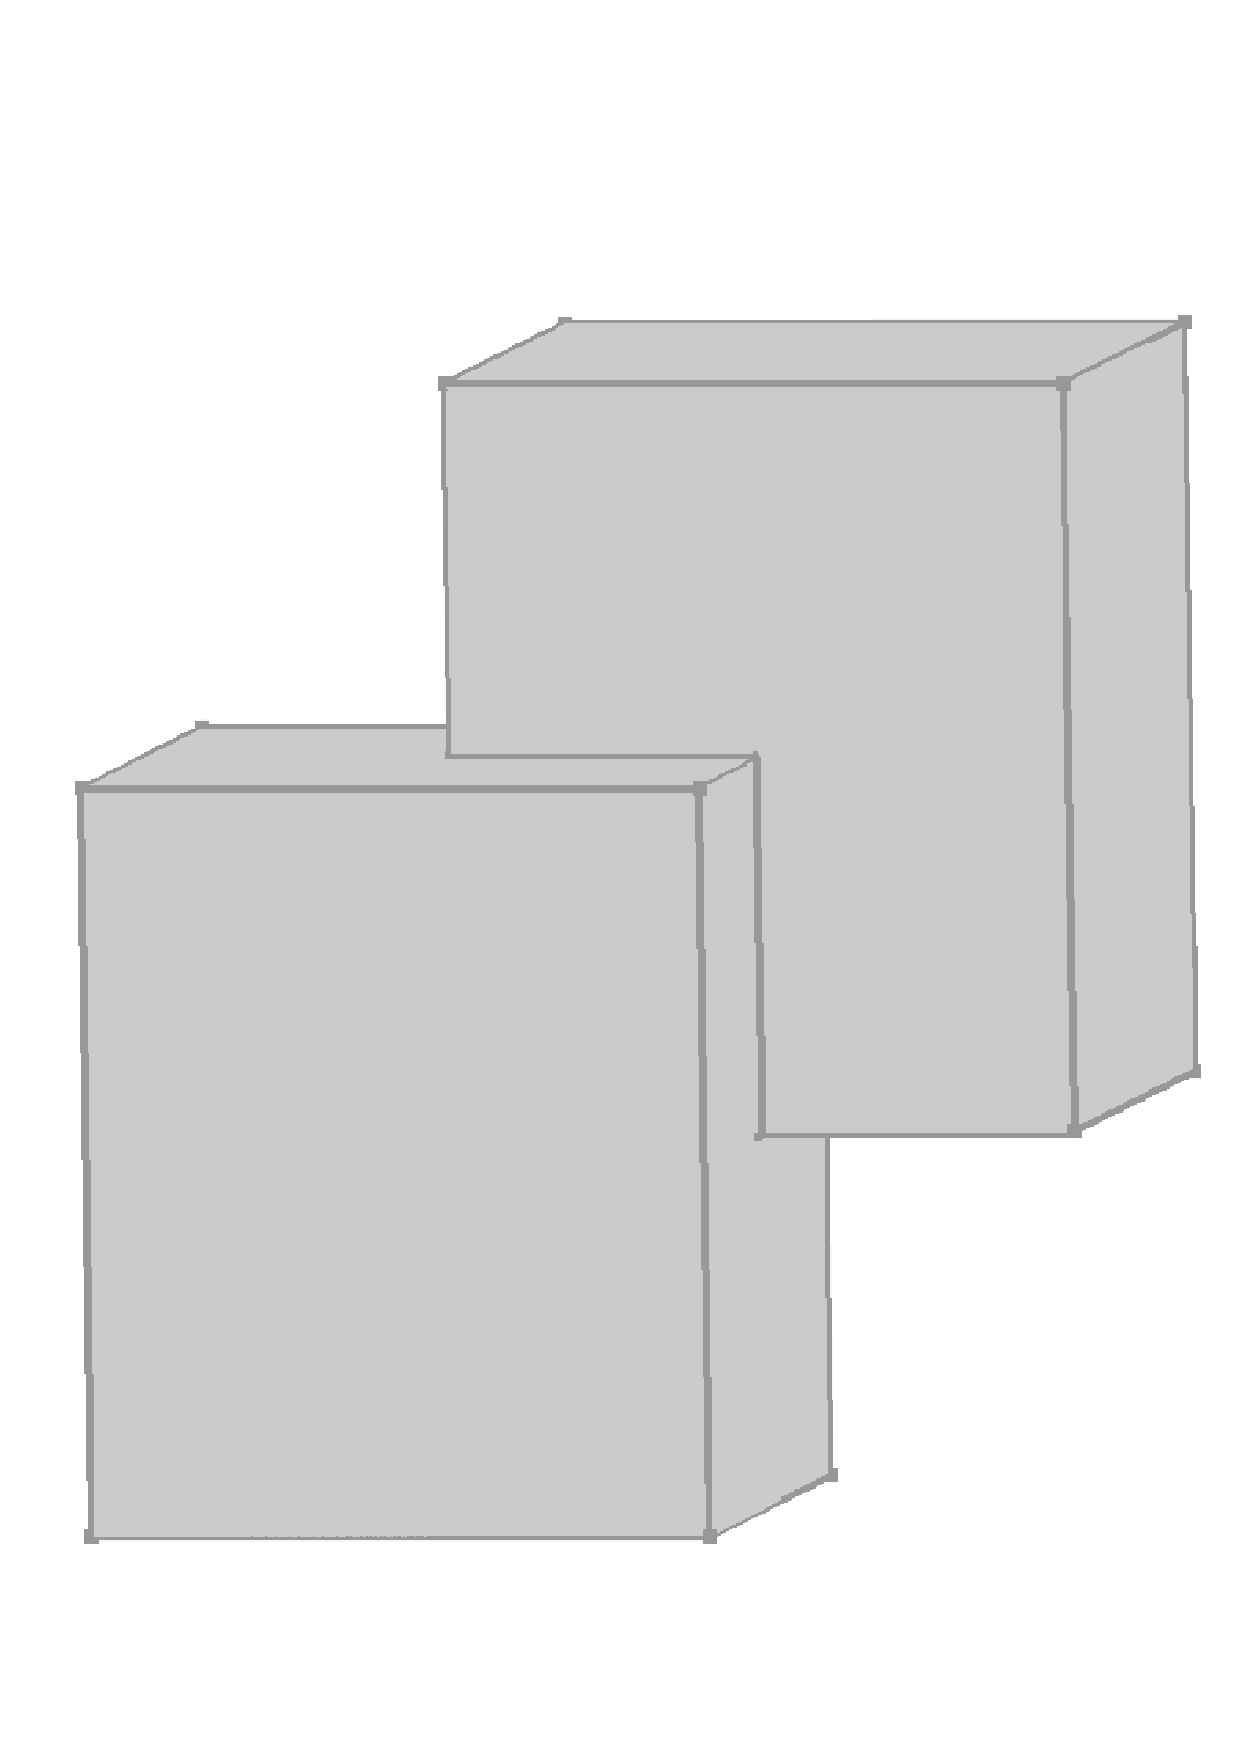
\includegraphics[width=0.245\textwidth]{Convex_decomposition_3/fig/two_cubes} \hspace{4mm}
      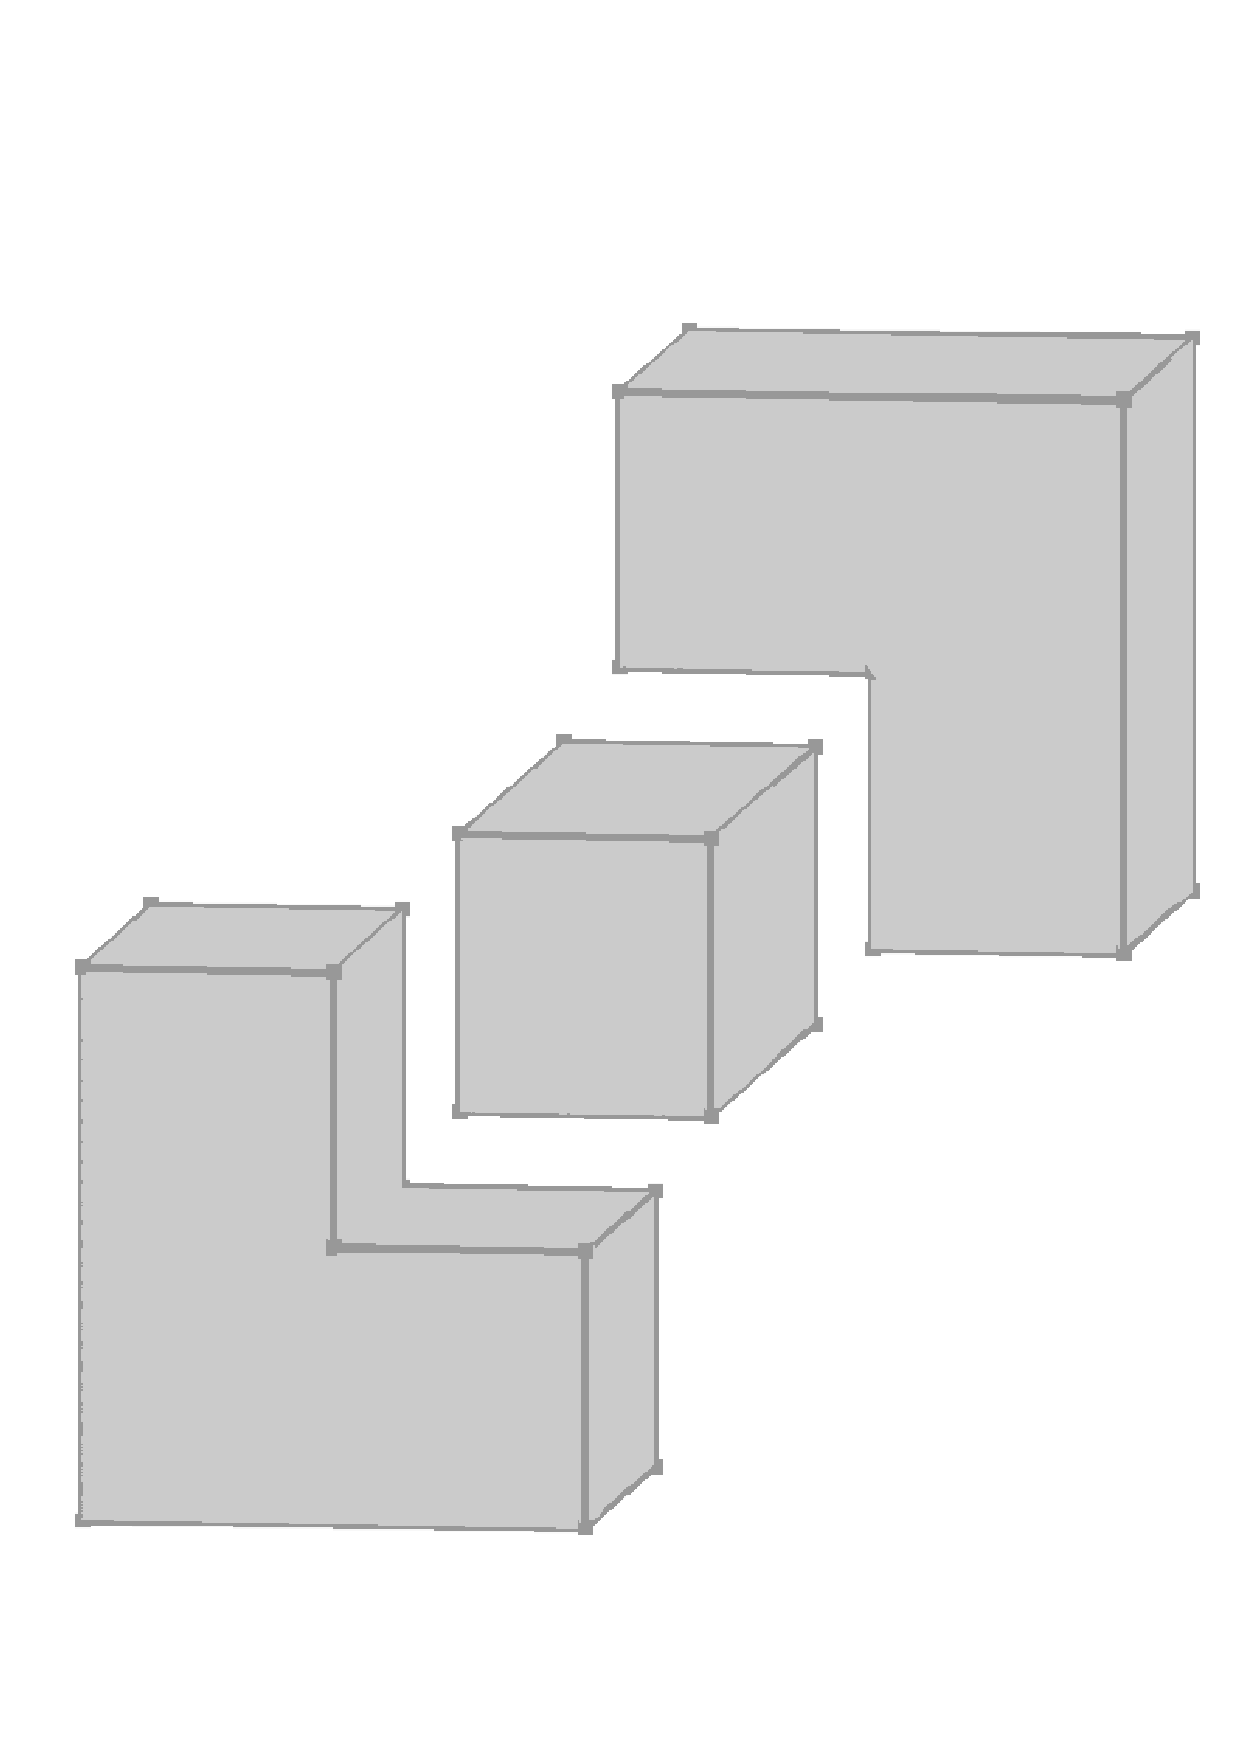
\includegraphics[width=0.25\textwidth]{Convex_decomposition_3/fig/two_cubes_cylindrical} \hspace{1mm}
      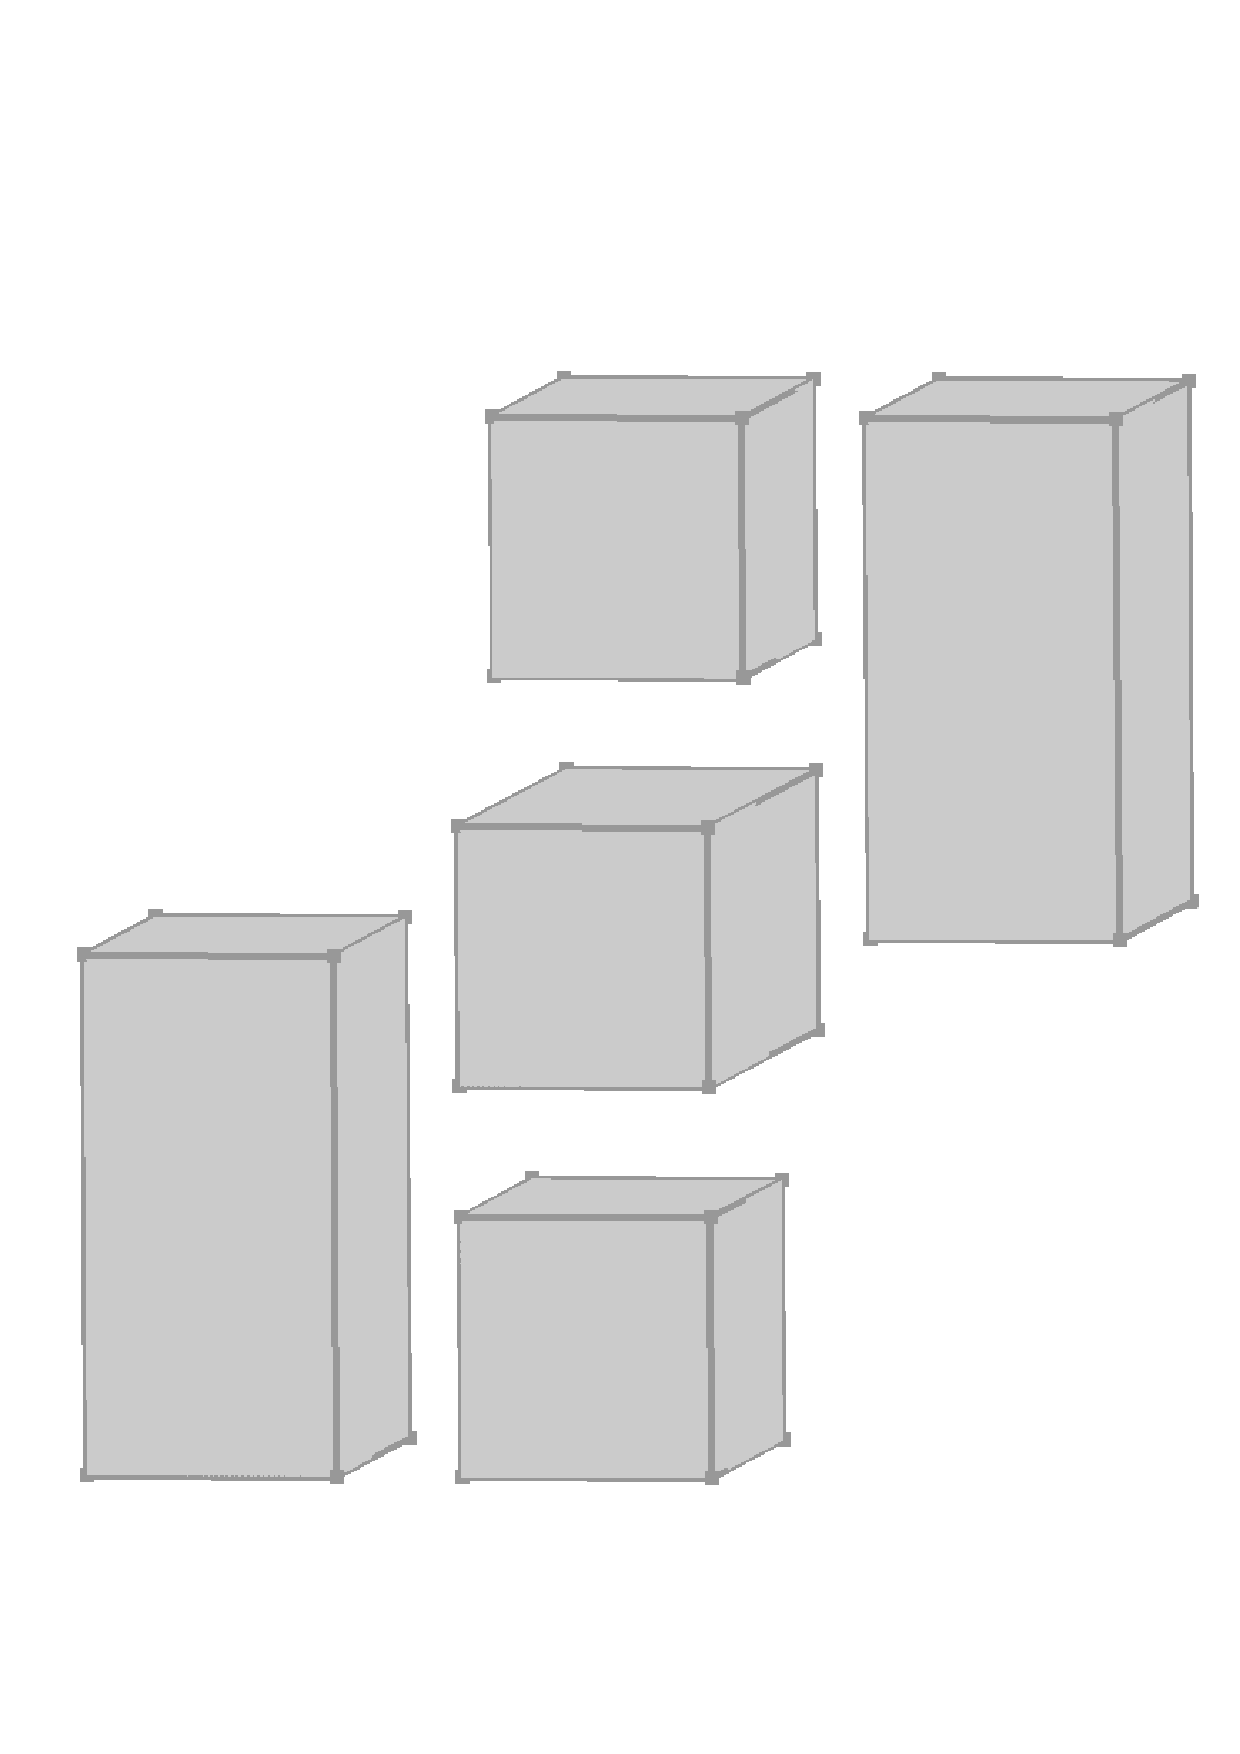
\includegraphics[width=0.27\textwidth]{Convex_decomposition_3/fig/two_cubes_vertical}
    \end{center}
  \end{ccTexOnly}
  \begin{ccHtmlOnly}
    <p><center>
    <img src="./fig/two_cubes.gif" border=0 alt="decomposition
    example" width=250>&nbsp;&nbsp;&nbsp;&nbsp;
    <img src="./fig/two_cubes_cylindrical.gif" border=0 alt="decomposition
    after first step" width=250>&nbsp;&nbsp;&nbsp;
    <img src="./fig/two_cubes_vertical.gif" border=0 alt="final
    decomposition" width=250>
    </center>
  \end{ccHtmlOnly}
  \caption{Vertical decomposition based on the insertion of vertical facets 
	   (viewed from the top). Left: Non-convex polyhedron. Middle:
	   Non-vertical reflex edges have been resolved. Right: Vertical
           reflex edges have been resolved. The sub-volumes are convex.}
  \label{fig:verticalDecomposition}
\end{figure}

Our decomposition runs in two steps. In the first step, each
non-vertical reflex edge $e$ is resolved by insertion of vertical
facets through $e$. In the second step, we do the same with the
vertical reflex edges. Figure~\ref{fig:verticalDecomposition}
illustrates the two steps.

At the moment our implementation is restricted to the decomposition of
bounded polyhedra. An extension to unbounded polyhedra is planned.

% +------------------------------------------------------------------------+
\section{Interface and Usage}

An instance of \ccc{Nef_polyhedron_3} represents a subdivision of the
three-dimensional space into vertices, edges, facets, and
volumes. Some of these items form the polyhedron (selected), while
others represent the outer volume or holes within the polyhedron
(unselected). As an example, the unit cube is the point set
$[0,1]^3$. The smallest subdivision that represents the unit cube has
8 vertices, 12 edges, 6 facets, and 2 volumes. The volumes enclosed by
the vertices, edges, and facets is the interior of the cube and
therefore selected. The volume outside the cube does not belong to it
and is therefore unselected. The vertices, edges, and facets---also
denoted as boundary items---are needed to separate the two volumes,
but are also useful for representing topological properties. In case
of the (closed) unit cube the boundary items are part of the
polyhedron and therefore selected, but in case of the open unit cube
$[0,1)^3$ they are unselected. Each item has its own selection mark,
which allows the correct representation of Nef polyhedra, which are
closed under Boolean and topological operations. Details can be found
in the chapter on 3D Boolean operations on Nef
polyhedra~\ref{chapterNef3}.

Usually, an instance of \ccc{Nef_polyhedron_3} does not contain any
redundant items. However, the function \ccc{convex_decomposition_3}
subdivides selected volumes of a given \ccc{Nef_polyhedron_3} by
selected facets. These additional facets are therefore redundant,
i.e., their insertion alters the representation of the polyhedron, but
not the polyhedron itself. 

When \ccc{convex_decomposition_3} resolved all reflex edges, the
selected sub-volumes have become convex. Each of them is represented
by a separate volume item and can therefore be traversed
separately~\ref{subsectionNef_3ShellExploration}. Another possibility
of accessing the convex pieces is to convert them into separate Nef
polyhedra, as illustrated by the example code given below.

Note that due to the restriction to bounded polyhedra, the use of
extended kernels is unnecessary and expensive. We therefore do not
support the use of extended kernels in the convex decomposition 
(see Chapter~\ref{chapterNef3}).

\ccIncludeExampleCode{Convex_decomposition_3/list_of_convex_parts.cpp}
